\documentclass[1p]{elsarticle_modified}
%\bibliographystyle{elsarticle-num}

%\usepackage[colorlinks]{hyperref}
%\usepackage{abbrmath_seonhwa} %\Abb, \Ascr, \Acal ,\Abf, \Afrak
\usepackage{amsfonts}
\usepackage{amssymb}
\usepackage{amsmath}
\usepackage{amsthm}
\usepackage{scalefnt}
\usepackage{amsbsy}
\usepackage{kotex}
\usepackage{caption}
\usepackage{subfig}
\usepackage{color}
\usepackage{graphicx}
\usepackage{xcolor} %% white, black, red, green, blue, cyan, magenta, yellow
\usepackage{float}
\usepackage{setspace}
\usepackage{hyperref}

\usepackage{tikz}
\usetikzlibrary{arrows}

\usepackage{multirow}
\usepackage{array} % fixed length table
\usepackage{hhline}

%%%%%%%%%%%%%%%%%%%%%
\makeatletter
\renewcommand*\env@matrix[1][\arraystretch]{%
	\edef\arraystretch{#1}%
	\hskip -\arraycolsep
	\let\@ifnextchar\new@ifnextchar
	\array{*\c@MaxMatrixCols c}}
\makeatother %https://tex.stackexchange.com/questions/14071/how-can-i-increase-the-line-spacing-in-a-matrix
%%%%%%%%%%%%%%%

\usepackage[normalem]{ulem}

\newcommand{\msout}[1]{\ifmmode\text{\sout{\ensuremath{#1}}}\else\sout{#1}\fi}
%SOURCE: \msout is \stkout macro in https://tex.stackexchange.com/questions/20609/strikeout-in-math-mode

\newcommand{\cancel}[1]{
	\ifmmode
	{\color{red}\msout{#1}}
	\else
	{\color{red}\sout{#1}}
	\fi
}

\newcommand{\add}[1]{
	{\color{blue}\uwave{#1}}
}

\newcommand{\replace}[2]{
	\ifmmode
	{\color{red}\msout{#1}}{\color{blue}\uwave{#2}}
	\else
	{\color{red}\sout{#1}}{\color{blue}\uwave{#2}}
	\fi
}

\newcommand{\Sol}{\mathcal{S}} %segment
\newcommand{\D}{D} %diagram
\newcommand{\A}{\mathcal{A}} %arc


%%%%%%%%%%%%%%%%%%%%%%%%%%%%%5 test

\def\sl{\operatorname{\textup{SL}}(2,\Cbb)}
\def\psl{\operatorname{\textup{PSL}}(2,\Cbb)}
\def\quan{\mkern 1mu \triangleright \mkern 1mu}

\theoremstyle{definition}
\newtheorem{thm}{Theorem}[section]
\newtheorem{prop}[thm]{Proposition}
\newtheorem{lem}[thm]{Lemma}
\newtheorem{ques}[thm]{Question}
\newtheorem{cor}[thm]{Corollary}
\newtheorem{defn}[thm]{Definition}
\newtheorem{exam}[thm]{Example}
\newtheorem{rmk}[thm]{Remark}
\newtheorem{alg}[thm]{Algorithm}

\newcommand{\I}{\sqrt{-1}}
\begin{document}

%\begin{frontmatter}
%
%\title{Boundary parabolic representations of knots up to 8 crossings}
%
%%% Group authors per affiliation:
%\author{Yunhi Cho} 
%\address{Department of Mathematics, University of Seoul, Seoul, Korea}
%\ead{yhcho@uos.ac.kr}
%
%
%\author{Seonhwa Kim} %\fnref{s_kim}}
%\address{Center for Geometry and Physics, Institute for Basic Science, Pohang, 37673, Korea}
%\ead{ryeona17@ibs.re.kr}
%
%\author{Hyuk Kim}
%\address{Department of Mathematical Sciences, Seoul National University, Seoul 08826, Korea}
%\ead{hyukkim@snu.ac.kr}
%
%\author{Seokbeom Yoon}
%\address{Department of Mathematical Sciences, Seoul National University, Seoul, 08826,  Korea}
%\ead{sbyoon15@snu.ac.kr}
%
%\begin{abstract}
%We find all boundary parabolic representation of knots up to 8 crossings.
%
%\end{abstract}
%\begin{keyword}
%    \MSC[2010] 57M25 
%\end{keyword}
%
%\end{frontmatter}

%\linenumbers
%\tableofcontents
%
\newcommand\colored[1]{\textcolor{white}{\rule[-0.35ex]{0.8em}{1.4ex}}\kern-0.8em\color{red} #1}%
%\newcommand\colored[1]{\textcolor{white}{ #1}\kern-2.17ex	\textcolor{white}{ #1}\kern-1.81ex	\textcolor{white}{ #1}\kern-2.15ex\color{red}#1	}

{\Large $\underline{12a_{0201}~(K12a_{0201})}$}

\setlength{\tabcolsep}{10pt}
\renewcommand{\arraystretch}{1.6}
\vspace{1cm}\begin{tabular}{m{100pt}>{\centering\arraybackslash}m{274pt}}
\multirow{5}{120pt}{
	\centering
	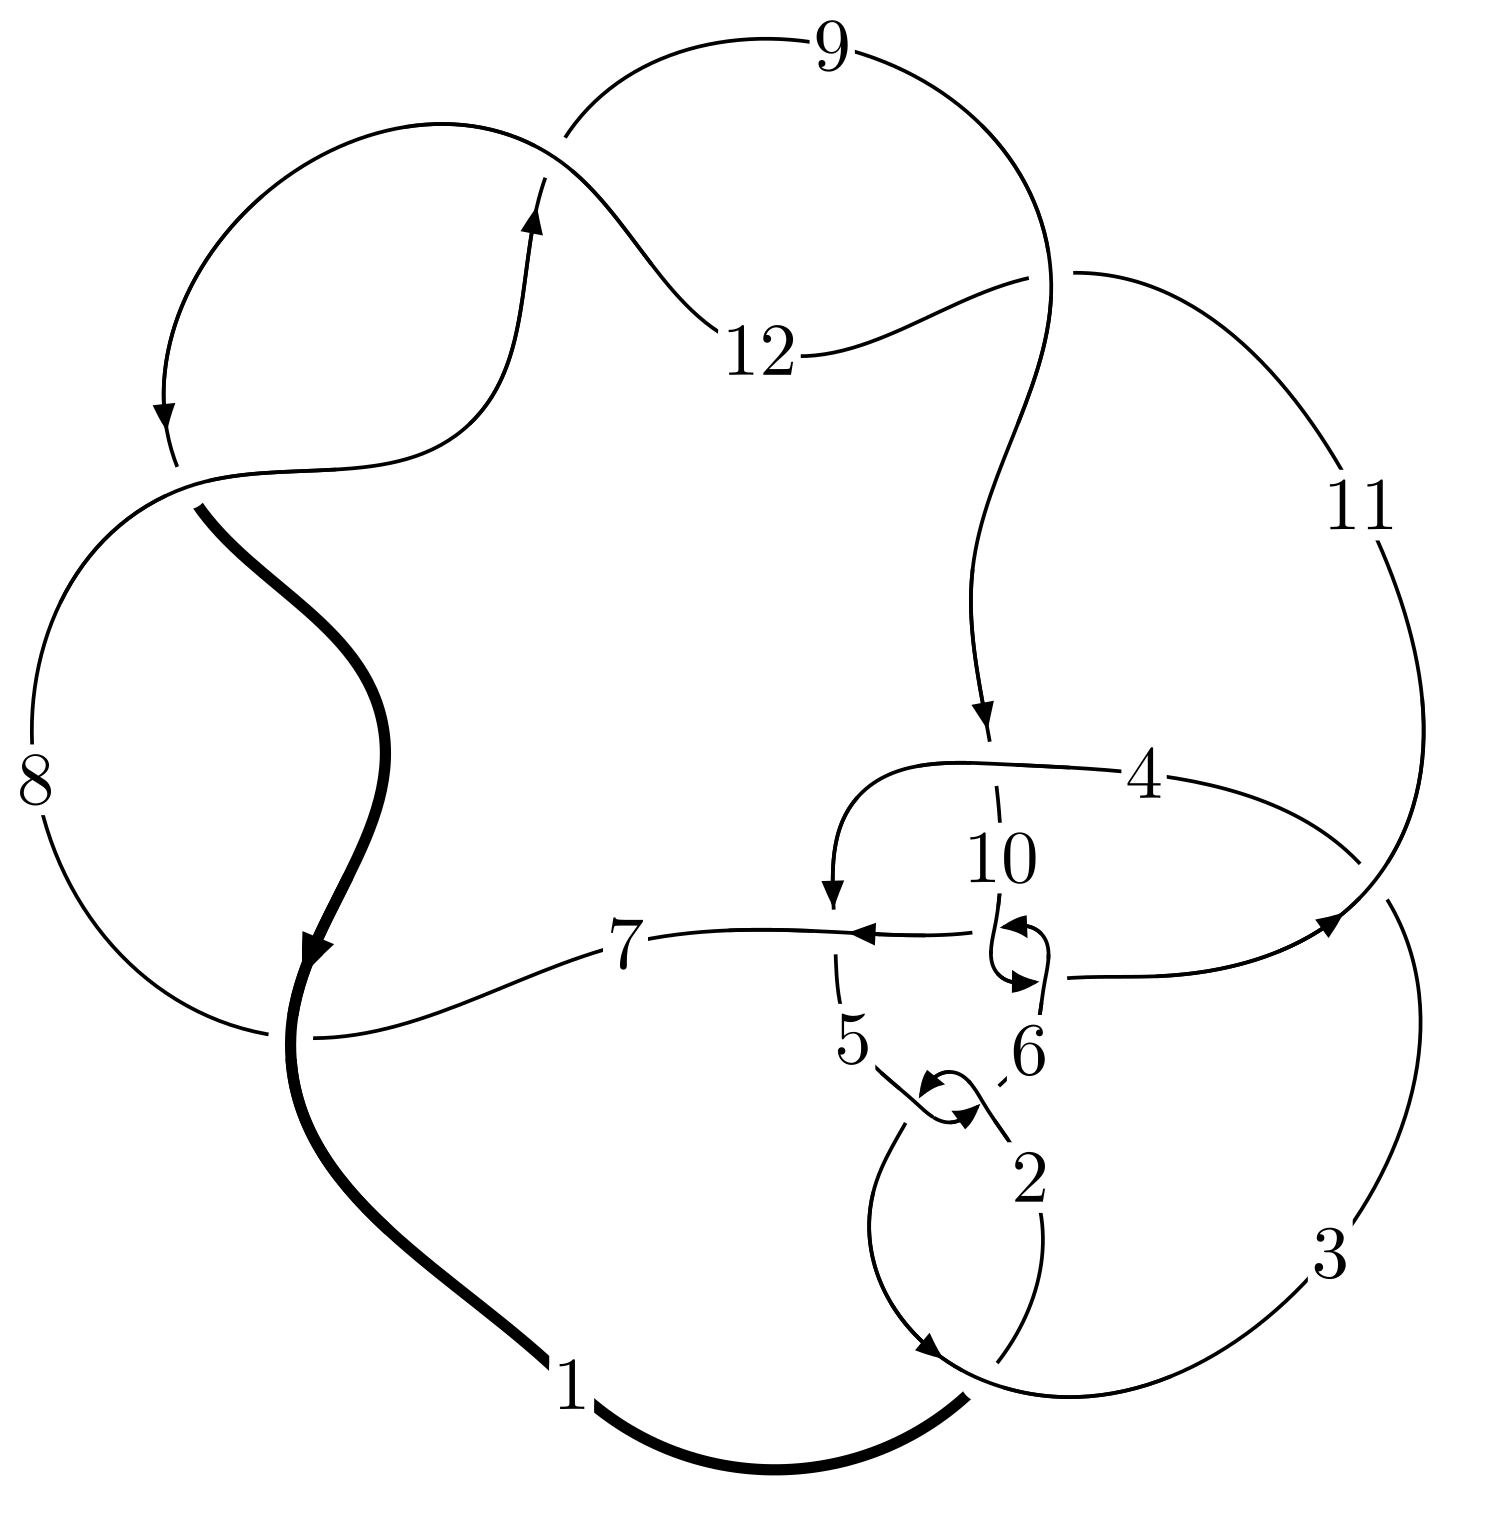
\includegraphics[width=112pt]{../../../GIT/diagram.site/Diagrams/png/1002_12a_0201.png}\\
\ \ \ A knot diagram\footnotemark}&
\allowdisplaybreaks
\textbf{Linearized knot diagam} \\
\cline{2-2}
 &
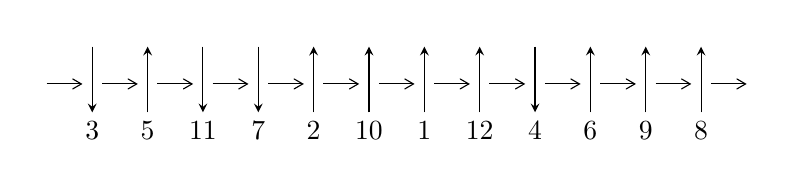
\begin{tikzpicture}[x=20pt, y=17pt]
	% nodes
	\node (C0) at (0, 0) {};
	\node (C1) at (1, 0) {};
	\node (C1U) at (1, +1) {};
	\node (C1D) at (1, -1) {3};

	\node (C2) at (2, 0) {};
	\node (C2U) at (2, +1) {};
	\node (C2D) at (2, -1) {5};

	\node (C3) at (3, 0) {};
	\node (C3U) at (3, +1) {};
	\node (C3D) at (3, -1) {11};

	\node (C4) at (4, 0) {};
	\node (C4U) at (4, +1) {};
	\node (C4D) at (4, -1) {7};

	\node (C5) at (5, 0) {};
	\node (C5U) at (5, +1) {};
	\node (C5D) at (5, -1) {2};

	\node (C6) at (6, 0) {};
	\node (C6U) at (6, +1) {};
	\node (C6D) at (6, -1) {10};

	\node (C7) at (7, 0) {};
	\node (C7U) at (7, +1) {};
	\node (C7D) at (7, -1) {1};

	\node (C8) at (8, 0) {};
	\node (C8U) at (8, +1) {};
	\node (C8D) at (8, -1) {12};

	\node (C9) at (9, 0) {};
	\node (C9U) at (9, +1) {};
	\node (C9D) at (9, -1) {4};

	\node (C10) at (10, 0) {};
	\node (C10U) at (10, +1) {};
	\node (C10D) at (10, -1) {6};

	\node (C11) at (11, 0) {};
	\node (C11U) at (11, +1) {};
	\node (C11D) at (11, -1) {9};

	\node (C12) at (12, 0) {};
	\node (C12U) at (12, +1) {};
	\node (C12D) at (12, -1) {8};
	\node (C13) at (13, 0) {};

	% arrows
	\draw[->,>={angle 60}]
	(C0) edge (C1) (C1) edge (C2) (C2) edge (C3) (C3) edge (C4) (C4) edge (C5) (C5) edge (C6) (C6) edge (C7) (C7) edge (C8) (C8) edge (C9) (C9) edge (C10) (C10) edge (C11) (C11) edge (C12) (C12) edge (C13) ;	\draw[->,>=stealth]
	(C1U) edge (C1D) (C2D) edge (C2U) (C3U) edge (C3D) (C4U) edge (C4D) (C5D) edge (C5U) (C6D) edge (C6U) (C7D) edge (C7U) (C8D) edge (C8U) (C9U) edge (C9D) (C10D) edge (C10U) (C11D) edge (C11U) (C12D) edge (C12U) ;
	\end{tikzpicture} \\
\hhline{~~} \\& 
\textbf{Solving Sequence} \\ \cline{2-2} 
 &
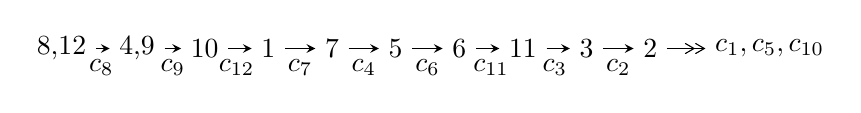
\begin{tikzpicture}[x=23pt, y=7pt]
	% node
	\node (A0) at (-1/8, 0) {8,12};
	\node (A1) at (17/16, 0) {4,9};
	\node (A2) at (17/8, 0) {10};
	\node (A3) at (25/8, 0) {1};
	\node (A4) at (33/8, 0) {7};
	\node (A5) at (41/8, 0) {5};
	\node (A6) at (49/8, 0) {6};
	\node (A7) at (57/8, 0) {11};
	\node (A8) at (65/8, 0) {3};
	\node (A9) at (73/8, 0) {2};
	\node (C1) at (1/2, -1) {$c_{8}$};
	\node (C2) at (13/8, -1) {$c_{9}$};
	\node (C3) at (21/8, -1) {$c_{12}$};
	\node (C4) at (29/8, -1) {$c_{7}$};
	\node (C5) at (37/8, -1) {$c_{4}$};
	\node (C6) at (45/8, -1) {$c_{6}$};
	\node (C7) at (53/8, -1) {$c_{11}$};
	\node (C8) at (61/8, -1) {$c_{3}$};
	\node (C9) at (69/8, -1) {$c_{2}$};
	\node (A10) at (11, 0) {$c_{1},c_{5},c_{10}$};

	% edge
	\draw[->,>=stealth]	
	(A0) edge (A1) (A1) edge (A2) (A2) edge (A3) (A3) edge (A4) (A4) edge (A5) (A5) edge (A6) (A6) edge (A7) (A7) edge (A8) (A8) edge (A9) ;
	\draw[->>,>={angle 60}]	
	(A9) edge (A10);
\end{tikzpicture} \\ 

\end{tabular} \\

\footnotetext{
The image of knot diagram is generated by the software ``\textbf{Draw programme}" developed by Andrew Bartholomew(\url{http://www.layer8.co.uk/maths/draw/index.htm\#Running-draw}), where we modified some parts for our purpose(\url{https://github.com/CATsTAILs/LinksPainter}).
}\phantom \\ \newline 
\centering \textbf{Ideals for irreducible components\footnotemark of $X_{\text{par}}$} 
 
\begin{align*}
I^u_{1}&=\langle 
-3.58867\times10^{91} u^{83}+1.02171\times10^{92} u^{82}+\cdots+1.57098\times10^{92} b-1.00231\times10^{92},\\
\phantom{I^u_{1}}&\phantom{= \langle  }-1.83263\times10^{92} u^{83}+5.48113\times10^{92} u^{82}+\cdots+1.57098\times10^{92} a+7.20038\times10^{92},\;u^{84}-3 u^{83}+\cdots-3 u+1\rangle \\
I^u_{2}&=\langle 
u^2 a+b,\;-10 u^2 a+25 a^2+5 a u+13 u^2-15 a+6 u+17,\;u^3+u^2+2 u+1\rangle \\
\\
\end{align*}
\raggedright * 2 irreducible components of $\dim_{\mathbb{C}}=0$, with total 90 representations.\\
\footnotetext{All coefficients of polynomials are rational numbers. But the coefficients are sometimes approximated in decimal forms when there is not enough margin.}
\newpage
\renewcommand{\arraystretch}{1}
\centering \section*{I. $I^u_{1}= \langle -3.59\times10^{91} u^{83}+1.02\times10^{92} u^{82}+\cdots+1.57\times10^{92} b-1.00\times10^{92},\;-1.83\times10^{92} u^{83}+5.48\times10^{92} u^{82}+\cdots+1.57\times10^{92} a+7.20\times10^{92},\;u^{84}-3 u^{83}+\cdots-3 u+1 \rangle$}
\flushleft \textbf{(i) Arc colorings}\\
\begin{tabular}{m{7pt} m{180pt} m{7pt} m{180pt} }
\flushright $a_{8}=$&$\begin{pmatrix}1\\0\end{pmatrix}$ \\
\flushright $a_{12}=$&$\begin{pmatrix}0\\u\end{pmatrix}$ \\
\flushright $a_{4}=$&$\begin{pmatrix}1.16655 u^{83}-3.48898 u^{82}+\cdots+6.40630 u-4.58336\\0.228435 u^{83}-0.650361 u^{82}+\cdots+0.796213 u+0.638014\end{pmatrix}$ \\
\flushright $a_{9}=$&$\begin{pmatrix}1\\- u^2\end{pmatrix}$ \\
\flushright $a_{10}=$&$\begin{pmatrix}0.00496120 u^{83}+0.0416024 u^{82}+\cdots-0.527099 u-0.844089\\0.0803009 u^{83}-0.303932 u^{82}+\cdots+0.736204 u+0.163754\end{pmatrix}$ \\
\flushright $a_{1}=$&$\begin{pmatrix}u\\u\end{pmatrix}$ \\
\flushright $a_{7}=$&$\begin{pmatrix}u^2+1\\u^2\end{pmatrix}$ \\
\flushright $a_{5}=$&$\begin{pmatrix}0.869710 u^{83}-2.51392 u^{82}+\cdots+3.61734 u-4.81101\\0.108064 u^{83}+0.181385 u^{82}+\cdots-0.185590 u+1.02410\end{pmatrix}$ \\
\flushright $a_{6}=$&$\begin{pmatrix}-0.163754 u^{83}+0.571563 u^{82}+\cdots-3.05646 u+1.22747\\-0.0564860 u^{83}+0.102861 u^{82}+\cdots+0.829205 u+0.00496120\end{pmatrix}$ \\
\flushright $a_{11}=$&$\begin{pmatrix}- u\\u^3+u\end{pmatrix}$ \\
\flushright $a_{3}=$&$\begin{pmatrix}0.835016 u^{83}-2.40727 u^{82}+\cdots+5.41664 u-4.56959\\0.175384 u^{83}-0.0477895 u^{82}+\cdots+1.19301 u+0.711354\end{pmatrix}$ \\
\flushright $a_{2}=$&$\begin{pmatrix}-0.667963 u^{83}+1.84046 u^{82}+\cdots-5.88896 u-1.51691\\-0.0928646 u^{83}+0.425791 u^{82}+\cdots+3.33040 u-0.355437\end{pmatrix}$\\&\end{tabular}
\flushleft \textbf{(ii) Obstruction class $= -1$}\\~\\
\flushleft \textbf{(iii) Cusp Shapes $= 2.16495 u^{83}-5.74232 u^{82}+\cdots+10.7785 u-2.44552$}\\~\\
\newpage\renewcommand{\arraystretch}{1}
\flushleft \textbf{(iv) u-Polynomials at the component}\newline \\
\begin{tabular}{m{50pt}|m{274pt}}
Crossings & \hspace{64pt}u-Polynomials at each crossing \\
\hline $$\begin{aligned}c_{1}\end{aligned}$$&$\begin{aligned}
&u^{84}+40 u^{83}+\cdots+3294 u+625
\end{aligned}$\\
\hline $$\begin{aligned}c_{2},c_{5}\end{aligned}$$&$\begin{aligned}
&u^{84}+4 u^{83}+\cdots+166 u+25
\end{aligned}$\\
\hline $$\begin{aligned}c_{3}\end{aligned}$$&$\begin{aligned}
&25(25 u^{84}+105 u^{83}+\cdots-18688 u+2563)
\end{aligned}$\\
\hline $$\begin{aligned}c_{4}\end{aligned}$$&$\begin{aligned}
&25(25 u^{84}+10 u^{83}+\cdots+227461 u+20617)
\end{aligned}$\\
\hline $$\begin{aligned}c_{6},c_{10}\end{aligned}$$&$\begin{aligned}
&u^{84}-3 u^{83}+\cdots-3 u+1
\end{aligned}$\\
\hline $$\begin{aligned}c_{7},c_{8},c_{11}\\c_{12}\end{aligned}$$&$\begin{aligned}
&u^{84}+3 u^{83}+\cdots+3 u+1
\end{aligned}$\\
\hline $$\begin{aligned}c_{9}\end{aligned}$$&$\begin{aligned}
&u^{84}- u^{83}+\cdots+8800 u+8000
\end{aligned}$\\
\hline
\end{tabular}\\~\\
\newpage\renewcommand{\arraystretch}{1}
\flushleft \textbf{(v) Riley Polynomials at the component}\newline \\
\begin{tabular}{m{50pt}|m{274pt}}
Crossings & \hspace{64pt}Riley Polynomials at each crossing \\
\hline $$\begin{aligned}c_{1}\end{aligned}$$&$\begin{aligned}
&y^{84}+12 y^{83}+\cdots-3086686 y+390625
\end{aligned}$\\
\hline $$\begin{aligned}c_{2},c_{5}\end{aligned}$$&$\begin{aligned}
&y^{84}+40 y^{83}+\cdots+3294 y+625
\end{aligned}$\\
\hline $$\begin{aligned}c_{3}\end{aligned}$$&$\begin{aligned}
&625(625 y^{84}-31725 y^{83}+\cdots-1.22498\times10^{8} y+6568969)
\end{aligned}$\\
\hline $$\begin{aligned}c_{4}\end{aligned}$$&$\begin{aligned}
&625(625 y^{84}-13650 y^{83}+\cdots-5.34301\times10^{10} y+4.25061\times10^{8})
\end{aligned}$\\
\hline $$\begin{aligned}c_{6},c_{10}\end{aligned}$$&$\begin{aligned}
&y^{84}+47 y^{83}+\cdots+19 y+1
\end{aligned}$\\
\hline $$\begin{aligned}c_{7},c_{8},c_{11}\\c_{12}\end{aligned}$$&$\begin{aligned}
&y^{84}+99 y^{83}+\cdots+19 y+1
\end{aligned}$\\
\hline $$\begin{aligned}c_{9}\end{aligned}$$&$\begin{aligned}
&y^{84}-35 y^{83}+\cdots-789120000 y+64000000
\end{aligned}$\\
\hline
\end{tabular}\\~\\
\newpage\flushleft \textbf{(vi) Complex Volumes and Cusp Shapes}
$$\begin{array}{c|c|c}  
\text{Solutions to }I^u_{1}& \I (\text{vol} + \sqrt{-1}CS) & \text{Cusp shape}\\
 \hline 
\begin{aligned}
u &= \phantom{-}0.559377 + 0.850834 I \\
a &= -1.34504 - 0.79140 I \\
b &= -0.0424165 + 0.1039430 I\end{aligned}
 & -5.4555 + 13.7745 I & \phantom{-0.000000 } 0 \\ \hline\begin{aligned}
u &= \phantom{-}0.559377 - 0.850834 I \\
a &= -1.34504 + 0.79140 I \\
b &= -0.0424165 - 0.1039430 I\end{aligned}
 & -5.4555 - 13.7745 I & \phantom{-0.000000 } 0 \\ \hline\begin{aligned}
u &= -0.603908 + 0.839047 I \\
a &= \phantom{-}0.818244 - 0.598416 I \\
b &= -0.0640806 + 0.0705229 I\end{aligned}
 & -1.66257 - 7.72348 I & \phantom{-0.000000 } 0 \\ \hline\begin{aligned}
u &= -0.603908 - 0.839047 I \\
a &= \phantom{-}0.818244 + 0.598416 I \\
b &= -0.0640806 - 0.0705229 I\end{aligned}
 & -1.66257 + 7.72348 I & \phantom{-0.000000 } 0 \\ \hline\begin{aligned}
u &= \phantom{-}0.354001 + 0.884267 I \\
a &= -1.44947 - 0.48407 I \\
b &= \phantom{-}0.151051 - 0.266514 I\end{aligned}
 & -8.77859 + 4.94528 I & \phantom{-0.000000 } 0 \\ \hline\begin{aligned}
u &= \phantom{-}0.354001 - 0.884267 I \\
a &= -1.44947 + 0.48407 I \\
b &= \phantom{-}0.151051 + 0.266514 I\end{aligned}
 & -8.77859 - 4.94528 I & \phantom{-0.000000 } 0 \\ \hline\begin{aligned}
u &= \phantom{-}0.501059 + 0.802771 I \\
a &= \phantom{-}1.45664 + 0.76972 I \\
b &= -0.0915011 - 0.0759455 I\end{aligned}
 & -3.02003 + 8.18197 I & \phantom{-0.000000 } 0 \\ \hline\begin{aligned}
u &= \phantom{-}0.501059 - 0.802771 I \\
a &= \phantom{-}1.45664 - 0.76972 I \\
b &= -0.0915011 + 0.0759455 I\end{aligned}
 & -3.02003 - 8.18197 I & \phantom{-0.000000 } 0 \\ \hline\begin{aligned}
u &= \phantom{-}0.575841 + 0.733284 I \\
a &= -0.084003 - 1.043710 I \\
b &= \phantom{-}0.182438 - 0.080722 I\end{aligned}
 & -7.12558 + 2.31715 I & \phantom{-0.000000 } 0 \\ \hline\begin{aligned}
u &= \phantom{-}0.575841 - 0.733284 I \\
a &= -0.084003 + 1.043710 I \\
b &= \phantom{-}0.182438 + 0.080722 I\end{aligned}
 & -7.12558 - 2.31715 I & \phantom{-0.000000 } 0\\
 \hline 
 \end{array}$$\newpage$$\begin{array}{c|c|c}  
\text{Solutions to }I^u_{1}& \I (\text{vol} + \sqrt{-1}CS) & \text{Cusp shape}\\
 \hline 
\begin{aligned}
u &= \phantom{-}0.352613 + 0.849364 I \\
a &= \phantom{-}0.561264 + 1.147210 I \\
b &= \phantom{-}0.162827 + 0.112680 I\end{aligned}
 & -3.83598 - 0.83646 I & \phantom{-0.000000 } 0 \\ \hline\begin{aligned}
u &= \phantom{-}0.352613 - 0.849364 I \\
a &= \phantom{-}0.561264 - 1.147210 I \\
b &= \phantom{-}0.162827 - 0.112680 I\end{aligned}
 & -3.83598 + 0.83646 I & \phantom{-0.000000 } 0 \\ \hline\begin{aligned}
u &= -0.059146 + 1.084560 I \\
a &= \phantom{-}0.794617 + 0.270479 I \\
b &= \phantom{-}0.322778 - 0.026997 I\end{aligned}
 & -3.51431 - 1.41708 I & \phantom{-0.000000 } 0 \\ \hline\begin{aligned}
u &= -0.059146 - 1.084560 I \\
a &= \phantom{-}0.794617 - 0.270479 I \\
b &= \phantom{-}0.322778 + 0.026997 I\end{aligned}
 & -3.51431 + 1.41708 I & \phantom{-0.000000 } 0 \\ \hline\begin{aligned}
u &= -0.505379 + 0.743093 I \\
a &= -0.966789 + 0.597818 I \\
b &= \phantom{-}0.0998708 + 0.0522679 I\end{aligned}
 & \phantom{-}0.26259 - 2.97021 I & \phantom{-0.000000 } 0 \\ \hline\begin{aligned}
u &= -0.505379 - 0.743093 I \\
a &= -0.966789 - 0.597818 I \\
b &= \phantom{-}0.0998708 - 0.0522679 I\end{aligned}
 & \phantom{-}0.26259 + 2.97021 I & \phantom{-0.000000 } 0 \\ \hline\begin{aligned}
u &= \phantom{-}0.498502 + 0.985151 I \\
a &= -0.394841 - 0.857254 I \\
b &= -0.080456 + 0.122688 I\end{aligned}
 & -6.24548 - 5.02549 I & \phantom{-0.000000 } 0 \\ \hline\begin{aligned}
u &= \phantom{-}0.498502 - 0.985151 I \\
a &= -0.394841 + 0.857254 I \\
b &= -0.080456 - 0.122688 I\end{aligned}
 & -6.24548 + 5.02549 I & \phantom{-0.000000 } 0 \\ \hline\begin{aligned}
u &= -0.823438 + 0.141577 I \\
a &= \phantom{-}0.235246 + 0.004564 I \\
b &= \phantom{-}0.607378 - 0.197816 I\end{aligned}
 & \phantom{-}0.48308 + 2.97342 I & \phantom{-0.000000 } 0 \\ \hline\begin{aligned}
u &= -0.823438 - 0.141577 I \\
a &= \phantom{-}0.235246 - 0.004564 I \\
b &= \phantom{-}0.607378 + 0.197816 I\end{aligned}
 & \phantom{-}0.48308 - 2.97342 I & \phantom{-0.000000 } 0\\
 \hline 
 \end{array}$$\newpage$$\begin{array}{c|c|c}  
\text{Solutions to }I^u_{1}& \I (\text{vol} + \sqrt{-1}CS) & \text{Cusp shape}\\
 \hline 
\begin{aligned}
u &= -0.350172 + 1.132160 I \\
a &= \phantom{-}0.625704 - 0.237671 I \\
b &= \phantom{-}0.198471 + 0.000769 I\end{aligned}
 & -3.54157 - 1.27620 I & \phantom{-0.000000 } 0 \\ \hline\begin{aligned}
u &= -0.350172 - 1.132160 I \\
a &= \phantom{-}0.625704 + 0.237671 I \\
b &= \phantom{-}0.198471 - 0.000769 I\end{aligned}
 & -3.54157 + 1.27620 I & \phantom{-0.000000 } 0 \\ \hline\begin{aligned}
u &= \phantom{-}0.774229 + 0.059652 I \\
a &= -0.319713 - 0.244575 I \\
b &= -0.930111 - 0.495675 I\end{aligned}
 & -3.06074 - 9.34032 I & \phantom{-}1.08705 + 7.00360 I \\ \hline\begin{aligned}
u &= \phantom{-}0.774229 - 0.059652 I \\
a &= -0.319713 + 0.244575 I \\
b &= -0.930111 + 0.495675 I\end{aligned}
 & -3.06074 + 9.34032 I & \phantom{-}1.08705 - 7.00360 I \\ \hline\begin{aligned}
u &= -0.057154 + 0.759277 I \\
a &= \phantom{-}2.92385 - 0.76517 I \\
b &= \phantom{-}1.44744 - 0.65670 I\end{aligned}
 & -2.74047 - 1.50981 I & -1.82977 + 7.34075 I \\ \hline\begin{aligned}
u &= -0.057154 - 0.759277 I \\
a &= \phantom{-}2.92385 + 0.76517 I \\
b &= \phantom{-}1.44744 + 0.65670 I\end{aligned}
 & -2.74047 + 1.50981 I & -1.82977 - 7.34075 I \\ \hline\begin{aligned}
u &= -0.283084 + 0.680233 I \\
a &= \phantom{-}0.176113 + 0.832722 I \\
b &= \phantom{-}0.305432 - 1.203210 I\end{aligned}
 & -3.10028 - 5.80914 I & -1.88912 + 10.77046 I \\ \hline\begin{aligned}
u &= -0.283084 - 0.680233 I \\
a &= \phantom{-}0.176113 - 0.832722 I \\
b &= \phantom{-}0.305432 + 1.203210 I\end{aligned}
 & -3.10028 + 5.80914 I & -1.88912 - 10.77046 I \\ \hline\begin{aligned}
u &= -0.663601 + 0.245565 I \\
a &= -0.299112 + 0.012132 I \\
b &= -0.426042 + 0.391408 I\end{aligned}
 & \phantom{-}1.80973 - 0.97588 I & \phantom{-}6.29958 - 0.92330 I \\ \hline\begin{aligned}
u &= -0.663601 - 0.245565 I \\
a &= -0.299112 - 0.012132 I \\
b &= -0.426042 - 0.391408 I\end{aligned}
 & \phantom{-}1.80973 + 0.97588 I & \phantom{-}6.29958 + 0.92330 I\\
 \hline 
 \end{array}$$\newpage$$\begin{array}{c|c|c}  
\text{Solutions to }I^u_{1}& \I (\text{vol} + \sqrt{-1}CS) & \text{Cusp shape}\\
 \hline 
\begin{aligned}
u &= \phantom{-}0.666820 + 0.079514 I \\
a &= \phantom{-}0.382678 + 0.101341 I \\
b &= \phantom{-}0.868529 + 0.564372 I\end{aligned}
 & -0.84887 - 4.24920 I & \phantom{-}4.48446 + 3.03882 I \\ \hline\begin{aligned}
u &= \phantom{-}0.666820 - 0.079514 I \\
a &= \phantom{-}0.382678 - 0.101341 I \\
b &= \phantom{-}0.868529 - 0.564372 I\end{aligned}
 & -0.84887 + 4.24920 I & \phantom{-}4.48446 - 3.03882 I \\ \hline\begin{aligned}
u &= \phantom{-}0.627872 + 0.171062 I \\
a &= -0.669086 + 0.483574 I \\
b &= -0.703760 + 0.442978 I\end{aligned}
 & -5.54769 + 1.76630 I & -2.07508 - 2.33583 I \\ \hline\begin{aligned}
u &= \phantom{-}0.627872 - 0.171062 I \\
a &= -0.669086 - 0.483574 I \\
b &= -0.703760 - 0.442978 I\end{aligned}
 & -5.54769 - 1.76630 I & -2.07508 + 2.33583 I \\ \hline\begin{aligned}
u &= \phantom{-}0.196060 + 0.617529 I \\
a &= \phantom{-}1.239230 - 0.333181 I \\
b &= -0.247349 - 1.018570 I\end{aligned}
 & -0.71568 + 3.16029 I & \phantom{-}2.36917 - 2.88022 I \\ \hline\begin{aligned}
u &= \phantom{-}0.196060 - 0.617529 I \\
a &= \phantom{-}1.239230 + 0.333181 I \\
b &= -0.247349 + 1.018570 I\end{aligned}
 & -0.71568 - 3.16029 I & \phantom{-}2.36917 + 2.88022 I \\ \hline\begin{aligned}
u &= -0.181114 + 0.588314 I \\
a &= -2.47298 + 3.00036 I \\
b &= -1.47689 + 0.99560 I\end{aligned}
 & -3.13471 + 1.93596 I & \phantom{-}4.26373 + 2.32250 I \\ \hline\begin{aligned}
u &= -0.181114 - 0.588314 I \\
a &= -2.47298 - 3.00036 I \\
b &= -1.47689 - 0.99560 I\end{aligned}
 & -3.13471 - 1.93596 I & \phantom{-}4.26373 - 2.32250 I \\ \hline\begin{aligned}
u &= -0.285706 + 1.360680 I \\
a &= -0.240060 + 0.370676 I \\
b &= -0.219517 + 0.162799 I\end{aligned}
 & -3.25781 - 4.38865 I & \phantom{-0.000000 } 0 \\ \hline\begin{aligned}
u &= -0.285706 - 1.360680 I \\
a &= -0.240060 - 0.370676 I \\
b &= -0.219517 - 0.162799 I\end{aligned}
 & -3.25781 + 4.38865 I & \phantom{-0.000000 } 0\\
 \hline 
 \end{array}$$\newpage$$\begin{array}{c|c|c}  
\text{Solutions to }I^u_{1}& \I (\text{vol} + \sqrt{-1}CS) & \text{Cusp shape}\\
 \hline 
\begin{aligned}
u &= \phantom{-}0.273958 + 0.517742 I \\
a &= \phantom{-}2.14473 + 0.91311 I \\
b &= -0.732241 - 0.347542 I\end{aligned}
 & -0.27546 + 3.96105 I & \phantom{-}3.31158 - 10.67062 I \\ \hline\begin{aligned}
u &= \phantom{-}0.273958 - 0.517742 I \\
a &= \phantom{-}2.14473 - 0.91311 I \\
b &= -0.732241 + 0.347542 I\end{aligned}
 & -0.27546 - 3.96105 I & \phantom{-}3.31158 + 10.67062 I \\ \hline\begin{aligned}
u &= -0.278794 + 0.406348 I \\
a &= -1.60602 + 0.57998 I \\
b &= \phantom{-}0.281917 + 0.460637 I\end{aligned}
 & \phantom{-}0.456460 - 1.219620 I & \phantom{-}6.20987 + 4.56453 I \\ \hline\begin{aligned}
u &= -0.278794 - 0.406348 I \\
a &= -1.60602 - 0.57998 I \\
b &= \phantom{-}0.281917 - 0.460637 I\end{aligned}
 & \phantom{-}0.456460 + 1.219620 I & \phantom{-}6.20987 - 4.56453 I \\ \hline\begin{aligned}
u &= -0.293880 + 0.377603 I \\
a &= -1.078430 - 0.084585 I \\
b &= \phantom{-}0.042583 + 0.717975 I\end{aligned}
 & \phantom{-}0.538633 - 1.103160 I & \phantom{-}7.21508 + 6.37604 I \\ \hline\begin{aligned}
u &= -0.293880 - 0.377603 I \\
a &= -1.078430 + 0.084585 I \\
b &= \phantom{-}0.042583 - 0.717975 I\end{aligned}
 & \phantom{-}0.538633 + 1.103160 I & \phantom{-}7.21508 - 6.37604 I \\ \hline\begin{aligned}
u &= -0.00893 + 1.56295 I \\
a &= \phantom{-}0.97735 + 1.24513 I \\
b &= \phantom{-}1.66511 + 1.48668 I\end{aligned}
 & -6.12688 - 1.59937 I & \phantom{-0.000000 } 0 \\ \hline\begin{aligned}
u &= -0.00893 - 1.56295 I \\
a &= \phantom{-}0.97735 - 1.24513 I \\
b &= \phantom{-}1.66511 - 1.48668 I\end{aligned}
 & -6.12688 + 1.59937 I & \phantom{-0.000000 } 0 \\ \hline\begin{aligned}
u &= -0.01945 + 1.57262 I \\
a &= \phantom{-}1.93490 + 0.40789 I \\
b &= \phantom{-}3.50479 + 0.31797 I\end{aligned}
 & -6.44558 - 1.79187 I & \phantom{-0.000000 } 0 \\ \hline\begin{aligned}
u &= -0.01945 - 1.57262 I \\
a &= \phantom{-}1.93490 - 0.40789 I \\
b &= \phantom{-}3.50479 - 0.31797 I\end{aligned}
 & -6.44558 + 1.79187 I & \phantom{-0.000000 } 0\\
 \hline 
 \end{array}$$\newpage$$\begin{array}{c|c|c}  
\text{Solutions to }I^u_{1}& \I (\text{vol} + \sqrt{-1}CS) & \text{Cusp shape}\\
 \hline 
\begin{aligned}
u &= \phantom{-}0.04000 + 1.57921 I \\
a &= -2.69888 - 0.37859 I \\
b &= -4.75339 - 0.35957 I\end{aligned}
 & -7.51330 + 4.86891 I & \phantom{-0.000000 } 0 \\ \hline\begin{aligned}
u &= \phantom{-}0.04000 - 1.57921 I \\
a &= -2.69888 + 0.37859 I \\
b &= -4.75339 + 0.35957 I\end{aligned}
 & -7.51330 - 4.86891 I & \phantom{-0.000000 } 0 \\ \hline\begin{aligned}
u &= -0.01120 + 1.58483 I \\
a &= -0.33329 - 1.70734 I \\
b &= -0.40623 - 4.78895 I\end{aligned}
 & -10.56600 + 1.42603 I & \phantom{-0.000000 } 0 \\ \hline\begin{aligned}
u &= -0.01120 - 1.58483 I \\
a &= -0.33329 + 1.70734 I \\
b &= -0.40623 + 4.78895 I\end{aligned}
 & -10.56600 - 1.42603 I & \phantom{-0.000000 } 0 \\ \hline\begin{aligned}
u &= \phantom{-}0.288131 + 0.291830 I \\
a &= -0.748039 - 1.103380 I \\
b &= \phantom{-}0.695579 + 0.725202 I\end{aligned}
 & \phantom{-}0.29629 - 1.71529 I & \phantom{-}6.13579 + 1.42425 I \\ \hline\begin{aligned}
u &= \phantom{-}0.288131 - 0.291830 I \\
a &= -0.748039 + 1.103380 I \\
b &= \phantom{-}0.695579 - 0.725202 I\end{aligned}
 & \phantom{-}0.29629 + 1.71529 I & \phantom{-}6.13579 - 1.42425 I \\ \hline\begin{aligned}
u &= \phantom{-}0.04376 + 1.60820 I \\
a &= -1.102070 - 0.442715 I \\
b &= -2.15482 + 0.08868 I\end{aligned}
 & -8.48978 + 3.97458 I & \phantom{-0.000000 } 0 \\ \hline\begin{aligned}
u &= \phantom{-}0.04376 - 1.60820 I \\
a &= -1.102070 + 0.442715 I \\
b &= -2.15482 - 0.08868 I\end{aligned}
 & -8.48978 - 3.97458 I & \phantom{-0.000000 } 0 \\ \hline\begin{aligned}
u &= -0.06572 + 1.61236 I \\
a &= \phantom{-}0.25388 - 1.78486 I \\
b &= \phantom{-}0.55057 - 2.45686 I\end{aligned}
 & -11.01890 - 7.03717 I & \phantom{-0.000000 } 0 \\ \hline\begin{aligned}
u &= -0.06572 - 1.61236 I \\
a &= \phantom{-}0.25388 + 1.78486 I \\
b &= \phantom{-}0.55057 + 2.45686 I\end{aligned}
 & -11.01890 + 7.03717 I & \phantom{-0.000000 } 0\\
 \hline 
 \end{array}$$\newpage$$\begin{array}{c|c|c}  
\text{Solutions to }I^u_{1}& \I (\text{vol} + \sqrt{-1}CS) & \text{Cusp shape}\\
 \hline 
\begin{aligned}
u &= -0.02406 + 1.63596 I \\
a &= -1.27658 + 1.06452 I \\
b &= -3.37497 + 3.38315 I\end{aligned}
 & -11.09410 - 1.87001 I & \phantom{-0.000000 } 0 \\ \hline\begin{aligned}
u &= -0.02406 - 1.63596 I \\
a &= -1.27658 - 1.06452 I \\
b &= -3.37497 - 3.38315 I\end{aligned}
 & -11.09410 + 1.87001 I & \phantom{-0.000000 } 0 \\ \hline\begin{aligned}
u &= \phantom{-}0.10980 + 1.63370 I \\
a &= -1.243870 - 0.667925 I \\
b &= -2.51489 - 1.49587 I\end{aligned}
 & -12.27640 + 0.94689 I & \phantom{-0.000000 } 0 \\ \hline\begin{aligned}
u &= \phantom{-}0.10980 - 1.63370 I \\
a &= -1.243870 + 0.667925 I \\
b &= -2.51489 + 1.49587 I\end{aligned}
 & -12.27640 - 0.94689 I & \phantom{-0.000000 } 0 \\ \hline\begin{aligned}
u &= -0.14236 + 1.63151 I \\
a &= \phantom{-}1.60169 - 0.04119 I \\
b &= \phantom{-}3.11449 - 0.09048 I\end{aligned}
 & -7.86900 - 5.39498 I & \phantom{-0.000000 } 0 \\ \hline\begin{aligned}
u &= -0.14236 - 1.63151 I \\
a &= \phantom{-}1.60169 + 0.04119 I \\
b &= \phantom{-}3.11449 + 0.09048 I\end{aligned}
 & -7.86900 + 5.39498 I & \phantom{-0.000000 } 0 \\ \hline\begin{aligned}
u &= \phantom{-}0.18027 + 1.63208 I \\
a &= \phantom{-}1.118390 + 0.583138 I \\
b &= \phantom{-}2.08381 + 1.15494 I\end{aligned}
 & -15.1614 + 5.2174 I & \phantom{-0.000000 } 0 \\ \hline\begin{aligned}
u &= \phantom{-}0.18027 - 1.63208 I \\
a &= \phantom{-}1.118390 - 0.583138 I \\
b &= \phantom{-}2.08381 - 1.15494 I\end{aligned}
 & -15.1614 - 5.2174 I & \phantom{-0.000000 } 0 \\ \hline\begin{aligned}
u &= \phantom{-}0.14361 + 1.64435 I \\
a &= -2.11765 - 0.04963 I \\
b &= -4.19419 - 0.00744 I\end{aligned}
 & -11.3977 + 10.6415 I & \phantom{-0.000000 } 0 \\ \hline\begin{aligned}
u &= \phantom{-}0.14361 - 1.64435 I \\
a &= -2.11765 + 0.04963 I \\
b &= -4.19419 + 0.00744 I\end{aligned}
 & -11.3977 - 10.6415 I & \phantom{-0.000000 } 0\\
 \hline 
 \end{array}$$\newpage$$\begin{array}{c|c|c}  
\text{Solutions to }I^u_{1}& \I (\text{vol} + \sqrt{-1}CS) & \text{Cusp shape}\\
 \hline 
\begin{aligned}
u &= \phantom{-}0.09631 + 1.66230 I \\
a &= \phantom{-}2.20269 - 0.24901 I \\
b &= \phantom{-}4.20217 - 0.38809 I\end{aligned}
 & -17.5922 + 6.6845 I & \phantom{-0.000000 } 0 \\ \hline\begin{aligned}
u &= \phantom{-}0.09631 - 1.66230 I \\
a &= \phantom{-}2.20269 + 0.24901 I \\
b &= \phantom{-}4.20217 + 0.38809 I\end{aligned}
 & -17.5922 - 6.6845 I & \phantom{-0.000000 } 0 \\ \hline\begin{aligned}
u &= -0.328502 + 0.059345 I \\
a &= \phantom{-}2.21199 - 2.70852 I \\
b &= -0.726650 - 0.503743 I\end{aligned}
 & -1.42146 + 3.57364 I & \phantom{-}4.61344 - 2.53748 I \\ \hline\begin{aligned}
u &= -0.328502 - 0.059345 I \\
a &= \phantom{-}2.21199 + 2.70852 I \\
b &= -0.726650 + 0.503743 I\end{aligned}
 & -1.42146 - 3.57364 I & \phantom{-}4.61344 + 2.53748 I \\ \hline\begin{aligned}
u &= -0.17610 + 1.65959 I \\
a &= -1.52509 + 0.08404 I \\
b &= -3.02998 + 0.08952 I\end{aligned}
 & -10.1779 - 10.7238 I & \phantom{-0.000000 } 0 \\ \hline\begin{aligned}
u &= -0.17610 - 1.65959 I \\
a &= -1.52509 - 0.08404 I \\
b &= -3.02998 - 0.08952 I\end{aligned}
 & -10.1779 + 10.7238 I & \phantom{-0.000000 } 0 \\ \hline\begin{aligned}
u &= \phantom{-}0.16399 + 1.66168 I \\
a &= \phantom{-}1.98755 + 0.07708 I \\
b &= \phantom{-}4.04967 + 0.09312 I\end{aligned}
 & -14.0467 + 16.5764 I & \phantom{-0.000000 } 0 \\ \hline\begin{aligned}
u &= \phantom{-}0.16399 - 1.66168 I \\
a &= \phantom{-}1.98755 - 0.07708 I \\
b &= \phantom{-}4.04967 - 0.09312 I\end{aligned}
 & -14.0467 - 16.5764 I & \phantom{-0.000000 } 0 \\ \hline\begin{aligned}
u &= \phantom{-}0.184110 + 0.262726 I \\
a &= -2.32875 - 0.09910 I \\
b &= \phantom{-}0.492273 + 0.447222 I\end{aligned}
 & \phantom{-}0.19160 - 1.53066 I & \phantom{-}0.415592 + 0.997580 I \\ \hline\begin{aligned}
u &= \phantom{-}0.184110 - 0.262726 I \\
a &= -2.32875 + 0.09910 I \\
b &= \phantom{-}0.492273 - 0.447222 I\end{aligned}
 & \phantom{-}0.19160 + 1.53066 I & \phantom{-}0.415592 - 0.997580 I\\
 \hline 
 \end{array}$$\newpage$$\begin{array}{c|c|c}  
\text{Solutions to }I^u_{1}& \I (\text{vol} + \sqrt{-1}CS) & \text{Cusp shape}\\
 \hline 
\begin{aligned}
u &= -0.07757 + 1.68352 I \\
a &= -1.51866 - 0.11008 I \\
b &= -3.13003 - 0.08518 I\end{aligned}
 & -13.07090 - 2.69496 I & \phantom{-0.000000 } 0 \\ \hline\begin{aligned}
u &= -0.07757 - 1.68352 I \\
a &= -1.51866 + 0.11008 I \\
b &= -3.13003 + 0.08518 I\end{aligned}
 & -13.07090 + 2.69496 I & \phantom{-0.000000 } 0 \\ \hline\begin{aligned}
u &= \phantom{-}0.10895 + 1.70761 I \\
a &= \phantom{-}1.271630 + 0.476012 I \\
b &= \phantom{-}2.67034 + 0.89787 I\end{aligned}
 & -15.7142 - 2.6891 I & \phantom{-0.000000 } 0 \\ \hline\begin{aligned}
u &= \phantom{-}0.10895 - 1.70761 I \\
a &= \phantom{-}1.271630 - 0.476012 I \\
b &= \phantom{-}2.67034 - 0.89787 I\end{aligned}
 & -15.7142 + 2.6891 I & \phantom{-0.000000 } 0\\
 \hline 
 \end{array}$$\newpage\newpage\renewcommand{\arraystretch}{1}
\centering \section*{II. $I^u_{2}= \langle u^2 a+b,\;-10 u^2 a+13 u^2+\cdots-15 a+17,\;u^3+u^2+2 u+1 \rangle$}
\flushleft \textbf{(i) Arc colorings}\\
\begin{tabular}{m{7pt} m{180pt} m{7pt} m{180pt} }
\flushright $a_{8}=$&$\begin{pmatrix}1\\0\end{pmatrix}$ \\
\flushright $a_{12}=$&$\begin{pmatrix}0\\u\end{pmatrix}$ \\
\flushright $a_{4}=$&$\begin{pmatrix}a\\- u^2 a\end{pmatrix}$ \\
\flushright $a_{9}=$&$\begin{pmatrix}1\\- u^2\end{pmatrix}$ \\
\flushright $a_{10}=$&$\begin{pmatrix}1\\- u^2\end{pmatrix}$ \\
\flushright $a_{1}=$&$\begin{pmatrix}u\\u\end{pmatrix}$ \\
\flushright $a_{7}=$&$\begin{pmatrix}u^2+1\\u^2\end{pmatrix}$ \\
\flushright $a_{5}=$&$\begin{pmatrix}2 a\\-2 u^2 a- a u\end{pmatrix}$ \\
\flushright $a_{6}=$&$\begin{pmatrix}- u\\- u\end{pmatrix}$ \\
\flushright $a_{11}=$&$\begin{pmatrix}- u\\- u^2- u-1\end{pmatrix}$ \\
\flushright $a_{3}=$&$\begin{pmatrix}u^2 a+a\\- u^2 a- a u- a\end{pmatrix}$ \\
\flushright $a_{2}=$&$\begin{pmatrix}u^2 a-\frac{4}{5} u^2+a+\frac{2}{5} u-\frac{6}{5}\\- u^2 a- a u+\frac{1}{5} u^2- a+\frac{7}{5} u+\frac{4}{5}\end{pmatrix}$\\&\end{tabular}
\flushleft \textbf{(ii) Obstruction class $= 1$}\\~\\
\flushleft \textbf{(iii) Cusp Shapes $= \frac{27}{5} u^2 a+\frac{74}{5} a u+\frac{87}{25} u^2+\frac{53}{5} a+\frac{94}{25} u+\frac{133}{25}$}\\~\\
\newpage\renewcommand{\arraystretch}{1}
\flushleft \textbf{(iv) u-Polynomials at the component}\newline \\
\begin{tabular}{m{50pt}|m{274pt}}
Crossings & \hspace{64pt}u-Polynomials at each crossing \\
\hline $$\begin{aligned}c_{1},c_{5}\end{aligned}$$&$\begin{aligned}
&(u^2- u+1)^3
\end{aligned}$\\
\hline $$\begin{aligned}c_{2}\end{aligned}$$&$\begin{aligned}
&(u^2+u+1)^3
\end{aligned}$\\
\hline $$\begin{aligned}c_{3}\end{aligned}$$&$\begin{aligned}
&25(25 u^6-20 u^5+21 u^4-6 u^3+5 u^2- u+1)
\end{aligned}$\\
\hline $$\begin{aligned}c_{4}\end{aligned}$$&$\begin{aligned}
&25(25 u^6-35 u^5+29 u^4-18 u^3+9 u^2-4 u+1)
\end{aligned}$\\
\hline $$\begin{aligned}c_{6}\end{aligned}$$&$\begin{aligned}
&(u^3- u^2+1)^2
\end{aligned}$\\
\hline $$\begin{aligned}c_{7},c_{8}\end{aligned}$$&$\begin{aligned}
&(u^3+u^2+2 u+1)^2
\end{aligned}$\\
\hline $$\begin{aligned}c_{9}\end{aligned}$$&$\begin{aligned}
&u^6
\end{aligned}$\\
\hline $$\begin{aligned}c_{10}\end{aligned}$$&$\begin{aligned}
&(u^3+u^2-1)^2
\end{aligned}$\\
\hline $$\begin{aligned}c_{11},c_{12}\end{aligned}$$&$\begin{aligned}
&(u^3- u^2+2 u-1)^2
\end{aligned}$\\
\hline
\end{tabular}\\~\\
\newpage\renewcommand{\arraystretch}{1}
\flushleft \textbf{(v) Riley Polynomials at the component}\newline \\
\begin{tabular}{m{50pt}|m{274pt}}
Crossings & \hspace{64pt}Riley Polynomials at each crossing \\
\hline $$\begin{aligned}c_{1},c_{2},c_{5}\end{aligned}$$&$\begin{aligned}
&(y^2+y+1)^3
\end{aligned}$\\
\hline $$\begin{aligned}c_{3}\end{aligned}$$&$\begin{aligned}
&625(625 y^6+650 y^5+451 y^4+184 y^3+55 y^2+9 y+1)
\end{aligned}$\\
\hline $$\begin{aligned}c_{4}\end{aligned}$$&$\begin{aligned}
&625(625 y^6+225 y^5+31 y^4-32 y^3-5 y^2+2 y+1)
\end{aligned}$\\
\hline $$\begin{aligned}c_{6},c_{10}\end{aligned}$$&$\begin{aligned}
&(y^3- y^2+2 y-1)^2
\end{aligned}$\\
\hline $$\begin{aligned}c_{7},c_{8},c_{11}\\c_{12}\end{aligned}$$&$\begin{aligned}
&(y^3+3 y^2+2 y-1)^2
\end{aligned}$\\
\hline $$\begin{aligned}c_{9}\end{aligned}$$&$\begin{aligned}
&y^6
\end{aligned}$\\
\hline
\end{tabular}\\~\\
\newpage\flushleft \textbf{(vi) Complex Volumes and Cusp Shapes}
$$\begin{array}{c|c|c}  
\text{Solutions to }I^u_{2}& \I (\text{vol} + \sqrt{-1}CS) & \text{Cusp shape}\\
 \hline 
\begin{aligned}
u &= -0.215080 + 1.307140 I \\
a &= -0.432147 - 0.224180 I \\
b &= -0.592331 - 0.615655 I\end{aligned}
 & -3.02413 - 4.85801 I & \phantom{-}2.36205 + 10.05749 I \\ \hline\begin{aligned}
u &= -0.215080 + 1.307140 I \\
a &= \phantom{-}0.410219 - 0.262160 I \\
b &= \phantom{-}0.829338 - 0.205146 I\end{aligned}
 & -3.02413 - 0.79824 I & \phantom{-}3.05664 - 3.74022 I \\ \hline\begin{aligned}
u &= -0.215080 - 1.307140 I \\
a &= -0.432147 + 0.224180 I \\
b &= -0.592331 + 0.615655 I\end{aligned}
 & -3.02413 + 4.85801 I & \phantom{-}2.36205 - 10.05749 I \\ \hline\begin{aligned}
u &= -0.215080 - 1.307140 I \\
a &= \phantom{-}0.410219 + 0.262160 I \\
b &= \phantom{-}0.829338 + 0.205146 I\end{aligned}
 & -3.02413 + 0.79824 I & \phantom{-}3.05664 + 3.74022 I \\ \hline\begin{aligned}
u &= -0.569840\phantom{ +0.000000I} \\
a &= \phantom{-}0.421928 + 0.730800 I \\
b &= -0.137007 - 0.237304 I\end{aligned}
 & \phantom{-}1.11345 - 2.02988 I & \phantom{-}5.96131 + 2.86462 I \\ \hline\begin{aligned}
u &= -0.569840\phantom{ +0.000000I} \\
a &= \phantom{-}0.421928 - 0.730800 I \\
b &= -0.137007 + 0.237304 I\end{aligned}
 & \phantom{-}1.11345 + 2.02988 I & \phantom{-}5.96131 - 2.86462 I\\
 \hline 
 \end{array}$$\newpage
\newpage\renewcommand{\arraystretch}{1}
\centering \section*{ III. u-Polynomials}
\begin{tabular}{m{50pt}|m{274pt}}
Crossings & \hspace{64pt}u-Polynomials at each crossing \\
\hline $$\begin{aligned}c_{1}\end{aligned}$$&$\begin{aligned}
&((u^2- u+1)^3)(u^{84}+40 u^{83}+\cdots+3294 u+625)
\end{aligned}$\\
\hline $$\begin{aligned}c_{2}\end{aligned}$$&$\begin{aligned}
&((u^2+u+1)^3)(u^{84}+4 u^{83}+\cdots+166 u+25)
\end{aligned}$\\
\hline $$\begin{aligned}c_{3}\end{aligned}$$&$\begin{aligned}
&625(25 u^6-20 u^5+21 u^4-6 u^3+5 u^2- u+1)\\
&\cdot(25 u^{84}+105 u^{83}+\cdots-18688 u+2563)
\end{aligned}$\\
\hline $$\begin{aligned}c_{4}\end{aligned}$$&$\begin{aligned}
&625(25 u^6-35 u^5+29 u^4-18 u^3+9 u^2-4 u+1)\\
&\cdot(25 u^{84}+10 u^{83}+\cdots+227461 u+20617)
\end{aligned}$\\
\hline $$\begin{aligned}c_{5}\end{aligned}$$&$\begin{aligned}
&((u^2- u+1)^3)(u^{84}+4 u^{83}+\cdots+166 u+25)
\end{aligned}$\\
\hline $$\begin{aligned}c_{6}\end{aligned}$$&$\begin{aligned}
&((u^3- u^2+1)^2)(u^{84}-3 u^{83}+\cdots-3 u+1)
\end{aligned}$\\
\hline $$\begin{aligned}c_{7},c_{8}\end{aligned}$$&$\begin{aligned}
&((u^3+u^2+2 u+1)^2)(u^{84}+3 u^{83}+\cdots+3 u+1)
\end{aligned}$\\
\hline $$\begin{aligned}c_{9}\end{aligned}$$&$\begin{aligned}
&u^6(u^{84}- u^{83}+\cdots+8800 u+8000)
\end{aligned}$\\
\hline $$\begin{aligned}c_{10}\end{aligned}$$&$\begin{aligned}
&((u^3+u^2-1)^2)(u^{84}-3 u^{83}+\cdots-3 u+1)
\end{aligned}$\\
\hline $$\begin{aligned}c_{11},c_{12}\end{aligned}$$&$\begin{aligned}
&((u^3- u^2+2 u-1)^2)(u^{84}+3 u^{83}+\cdots+3 u+1)
\end{aligned}$\\
\hline
\end{tabular}\newpage\renewcommand{\arraystretch}{1}
\centering \section*{ IV. Riley Polynomials}
\begin{tabular}{m{50pt}|m{274pt}}
Crossings & \hspace{64pt}Riley Polynomials at each crossing \\
\hline $$\begin{aligned}c_{1}\end{aligned}$$&$\begin{aligned}
&((y^2+y+1)^3)(y^{84}+12 y^{83}+\cdots-3086686 y+390625)
\end{aligned}$\\
\hline $$\begin{aligned}c_{2},c_{5}\end{aligned}$$&$\begin{aligned}
&((y^2+y+1)^3)(y^{84}+40 y^{83}+\cdots+3294 y+625)
\end{aligned}$\\
\hline $$\begin{aligned}c_{3}\end{aligned}$$&$\begin{aligned}
&390625(625 y^6+650 y^5+451 y^4+184 y^3+55 y^2+9 y+1)\\
&\cdot(625 y^{84}-31725 y^{83}+\cdots-122497860 y+6568969)
\end{aligned}$\\
\hline $$\begin{aligned}c_{4}\end{aligned}$$&$\begin{aligned}
&390625(625 y^6+225 y^5+31 y^4-32 y^3-5 y^2+2 y+1)\\
&\cdot(625 y^{84}-13650 y^{83}+\cdots-53430131371 y+425060689)
\end{aligned}$\\
\hline $$\begin{aligned}c_{6},c_{10}\end{aligned}$$&$\begin{aligned}
&((y^3- y^2+2 y-1)^2)(y^{84}+47 y^{83}+\cdots+19 y+1)
\end{aligned}$\\
\hline $$\begin{aligned}c_{7},c_{8},c_{11}\\c_{12}\end{aligned}$$&$\begin{aligned}
&((y^3+3 y^2+2 y-1)^2)(y^{84}+99 y^{83}+\cdots+19 y+1)
\end{aligned}$\\
\hline $$\begin{aligned}c_{9}\end{aligned}$$&$\begin{aligned}
&y^6(y^{84}-35 y^{83}+\cdots-7.89120\times10^{8} y+6.40000\times10^{7})
\end{aligned}$\\
\hline
\end{tabular}
\vskip 2pc
\end{document}